\begin{figure}
    \begin{center}
    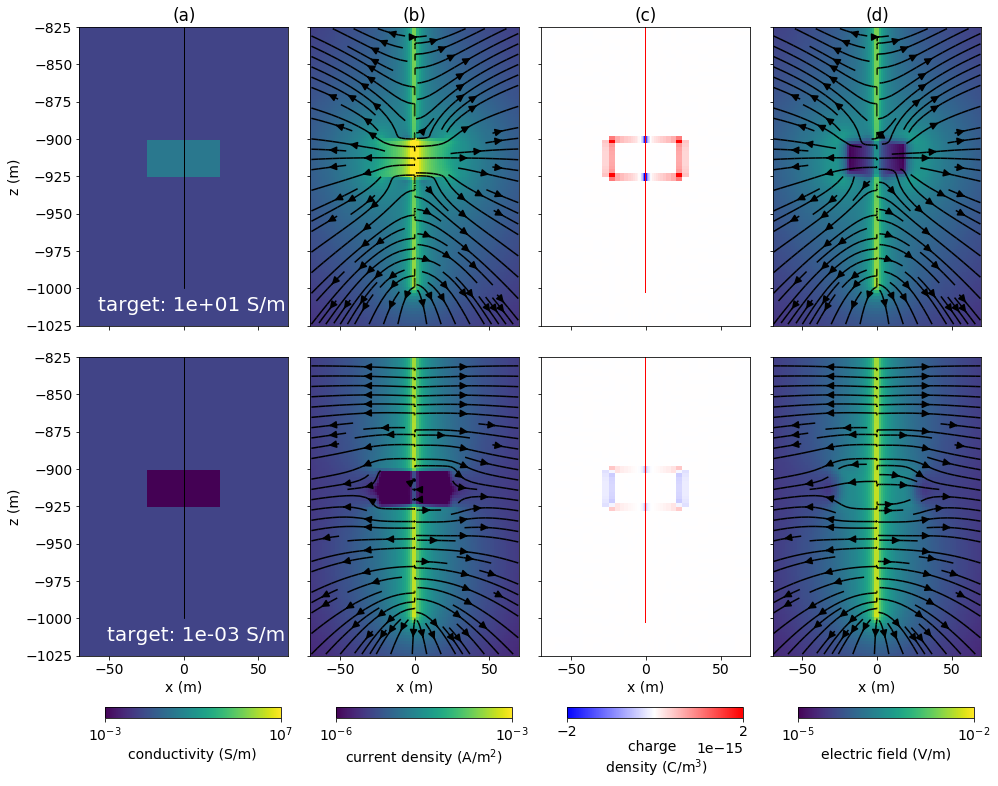
\includegraphics[width=\textwidth]{figures/offset_target_physics.png}
    \end{center}
\caption{
    Cross section showing: (a) electrical conductivity, (b) current density, (c) charge density, and
    (d) electric field for a DC resistivity experiment with a conductive target (top)
    and a resistive target (bottom) which is not in contact with the well.
    The positive electrode is positioned in the casing at the 912.5m depth.
    The casing is shown by the black line that extends to 1km
    depth in panel (a).
}
\label{fig:offset_target_physics}
\end{figure}
